\documentclass{main.tex}[subfiles]
\begin{document}
\newpage
\nonumsection{Приложение 1. Дополнительные иллюстрации}

%\begin{figure}[H]
%    \centering
%    \includegraphics[width=\myPictWidth]{ovodov_forum}
%    \caption{И.Г. Оводов представляет проект распознавания шрифта Брайля по фотографии на форуме <<Сильные идеи для нового времени>>. Кадр телеканала <<Россия 24>> \protect\footnotemark}
%    \label{fig:ovodov_forum}
%\end{figure}
%
%\footnotetext{\href{https://youtu.be/SVocn-tnjz8?t=5427}{Форум АСИ "Сильные идеи для нового времени". Полная версия (YouTube)}}

\begin{figure}[H]
    \centering
    \begin{subfigure}{.5\textwidth}
        \centering
        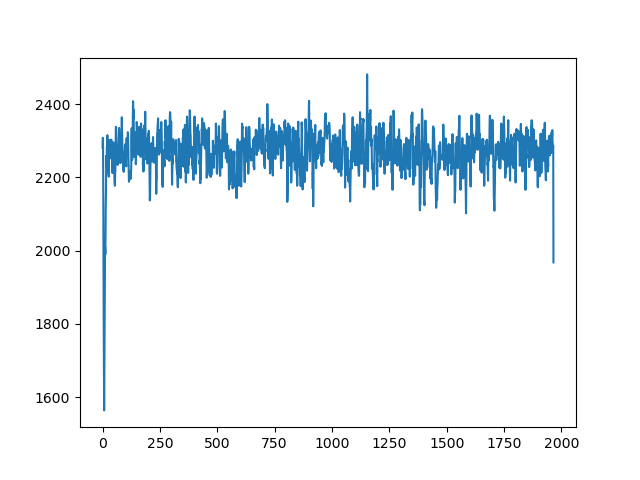
\includegraphics[width=\myPictWidth]{test_find_regions/find_regions_k2}
        \caption{$ k = 2 $}
        % TODO \label{fig:}
    \end{subfigure}%
    \begin{subfigure}{.5\textwidth}
        \centering
        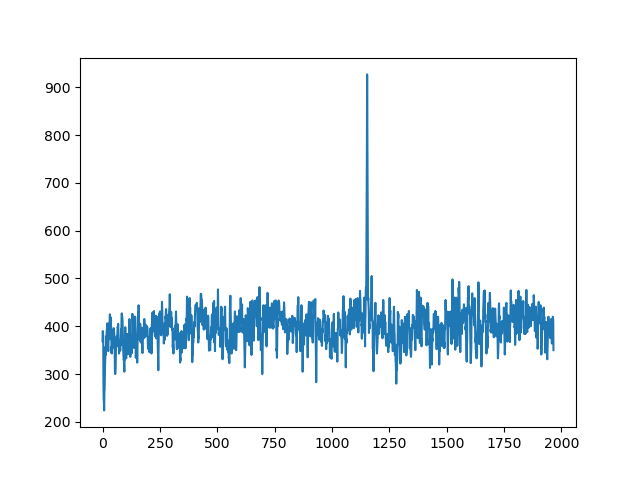
\includegraphics[width=\myPictWidth]{test_find_regions/find_regions_k4}
        \caption{$ k = 4 $}
        % TODO \label{fig:}
    \end{subfigure}

    \begin{subfigure}{.5\textwidth}
        \centering
        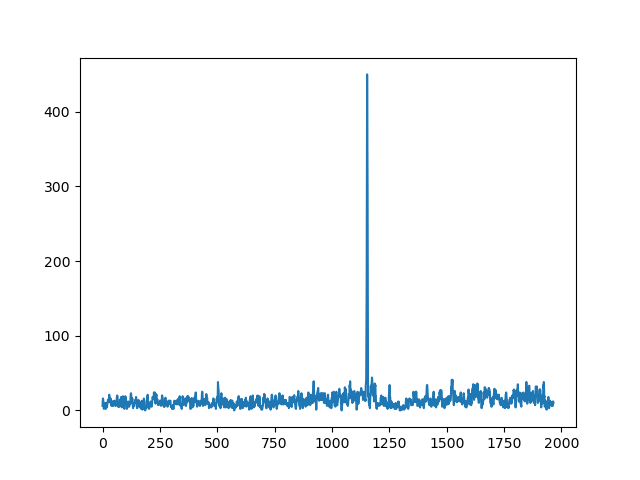
\includegraphics[width=\myPictWidth]{test_find_regions/find_regions_k8}
        \caption{$ k = 8 $}
        % TODO \label{fig:}
    \end{subfigure}%
    \begin{subfigure}{.5\textwidth}
        \centering
        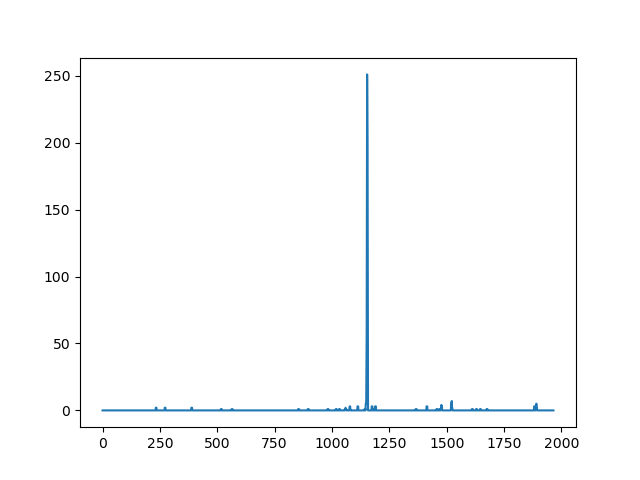
\includegraphics[width=\myPictWidth]{test_find_regions/find_regions_k15}
        \caption{$ k = 15 $}
        % TODO \label{fig:}
    \end{subfigure}
    \caption{Зависимость числа k-грам, найденных в регионе исходного текста, от позиции региона относительно начала текста}
    \label{fig:find_k}
\end{figure}

\begin{figure}[H]
    \centering
    \begin{subfigure}{.5\textwidth}
        \centering
        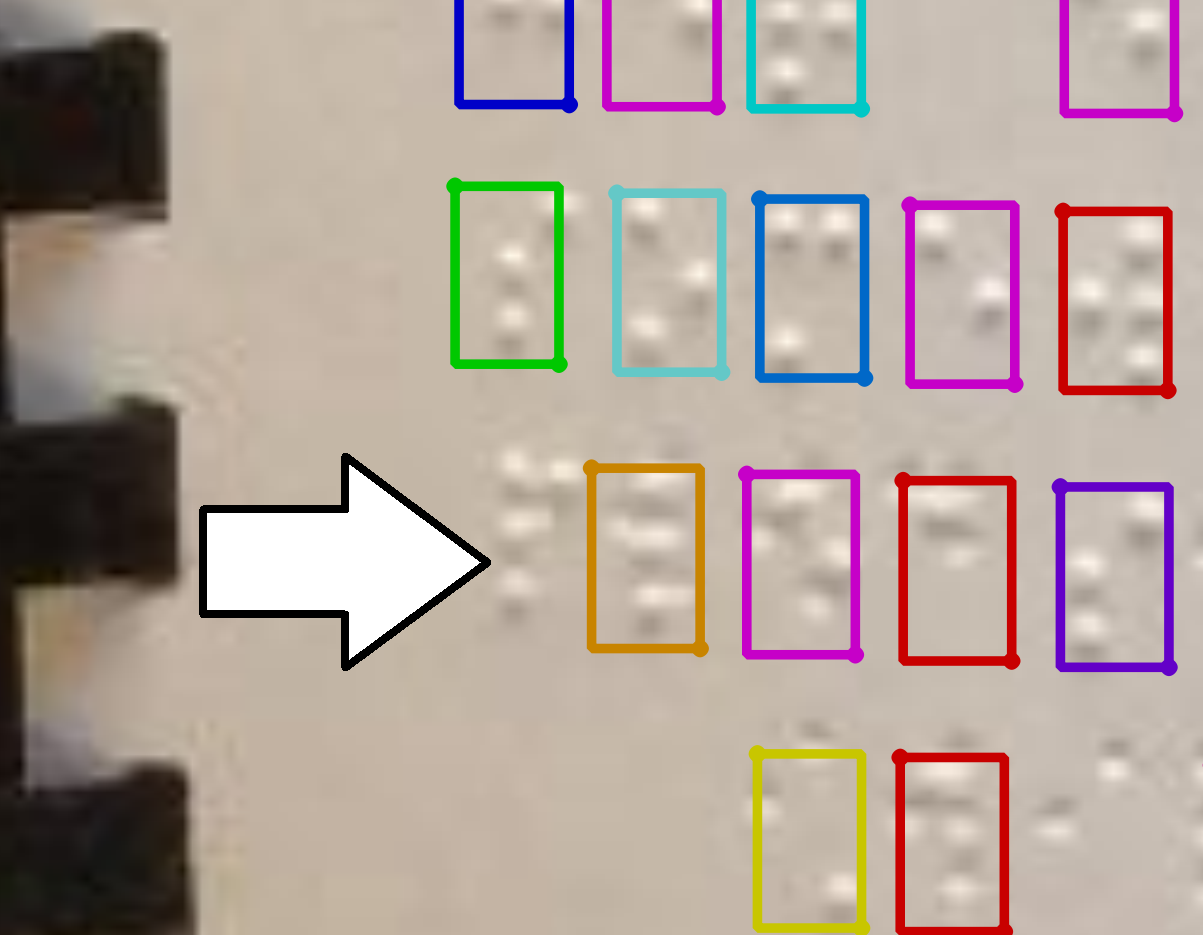
\includegraphics[width=.95\myPictWidth]{recogn_mistakes/deletion}
        \caption{Выпадение символа}
        \label{fig:recogn_mistakes:del}
    \end{subfigure}%
    \begin{subfigure}{.5\textwidth}
        \centering
        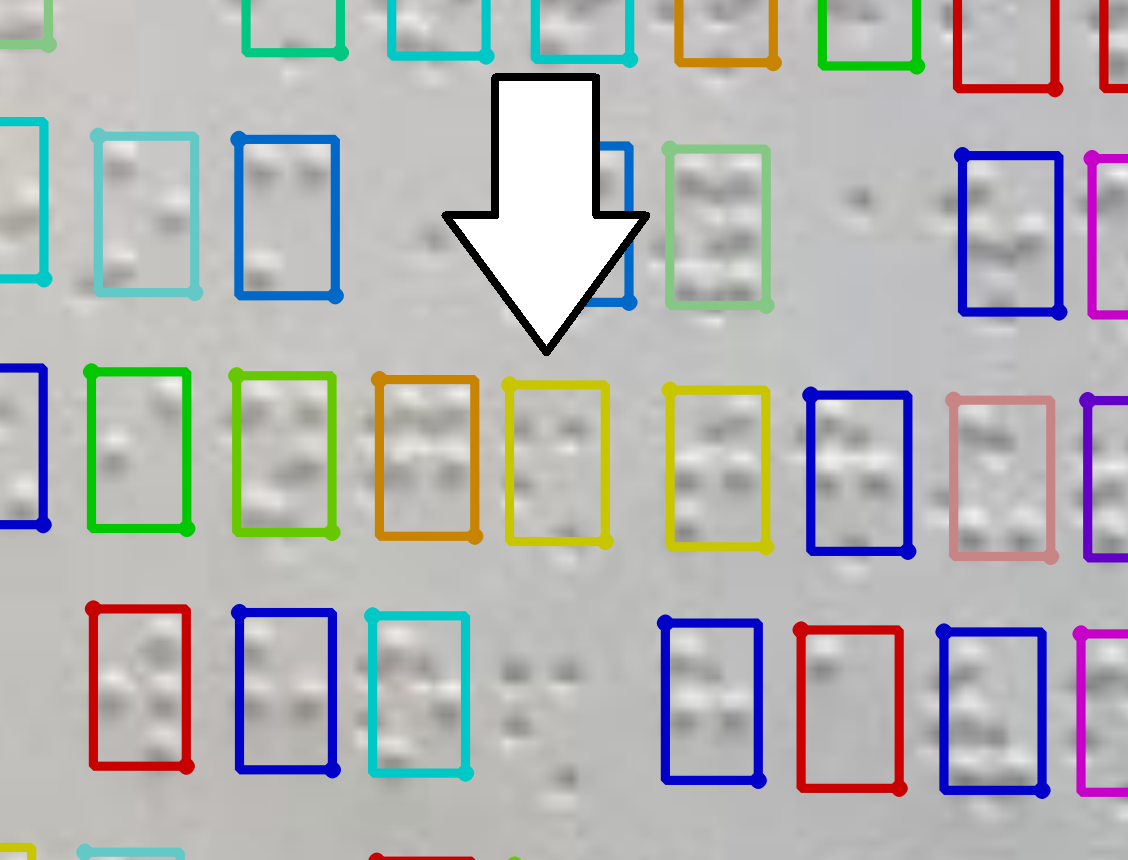
\includegraphics[width=.95\myPictWidth]{recogn_mistakes/insertion}
        \caption{Вставка символа}
        \label{fig:recogn_mistakes:ins}
    \end{subfigure}

    \begin{subfigure}{.5\textwidth}
        \centering
        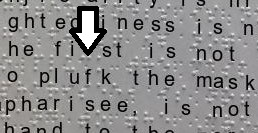
\includegraphics[width=.95\myPictWidth]{recogn_mistakes/mismatch}
        \caption{Неверно распознан символ}
        \label{fig:recogn_mistakes:mismatch}
    \end{subfigure}%
    \begin{subfigure}{.5\textwidth}
        \centering
        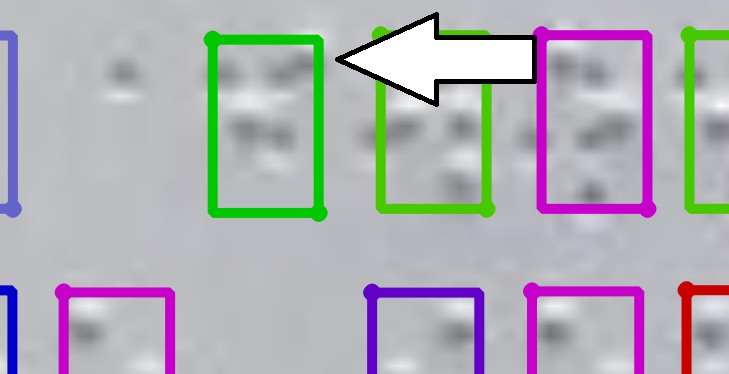
\includegraphics[width=.95\myPictWidth]{recogn_mistakes/misplaced_label}
        \caption{Неверно обозначены границы объекта}
        \label{fig:recogn_mistakes:misplaced_label}
    \end{subfigure}
    \caption{Разновидности ошибок распознавания}
    \label{fig:recogn_mistakes}
\end{figure}

\begin{figure}[H]
    \centering
    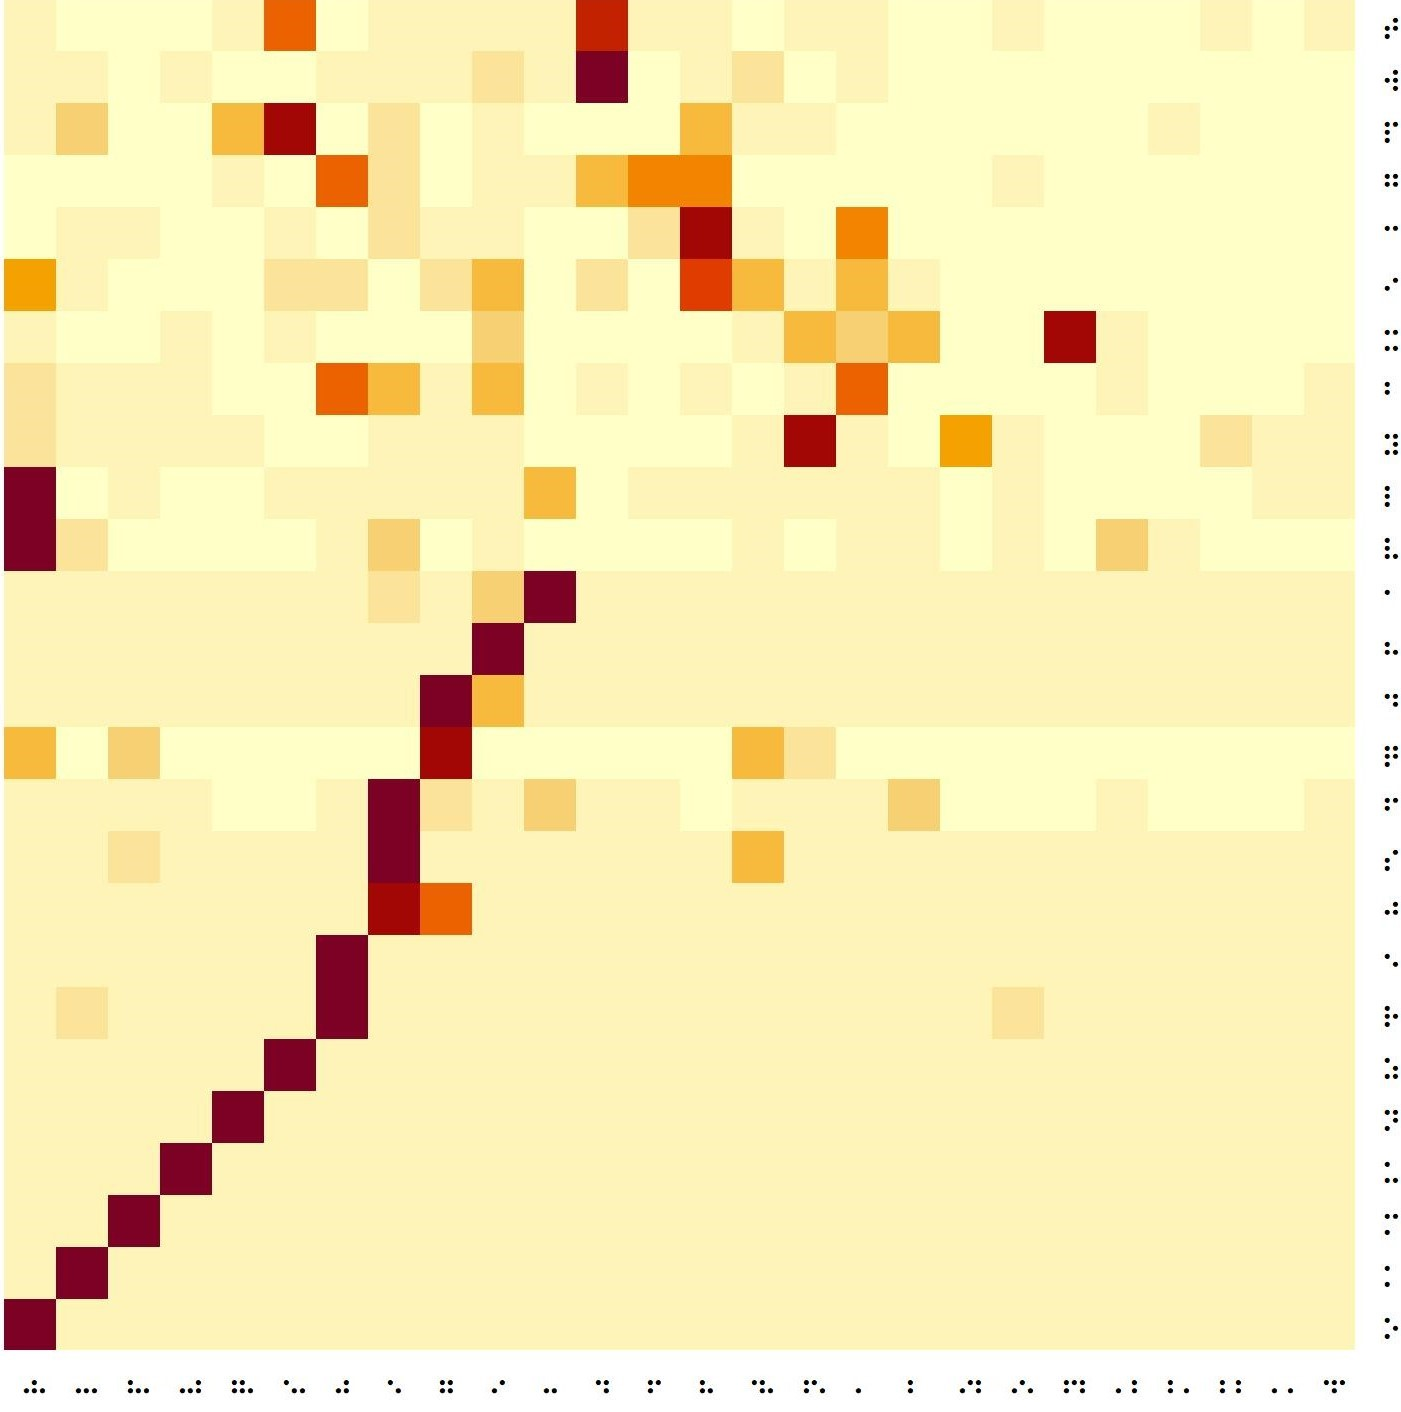
\includegraphics[width=\myPictWidth]{errors_stats/heatmap_alphabet}
    \caption{Частоты замен букв на другие буквы (по вертикали -- верный символ, записанный шрифтом Брайля, по горизонтали -- распознанный). Цвет показывает долю исходных символов, приходящихся на заменяемый (чем темнее, тем больше). Верно распознанные буквы не учтены.}
    \label{fig:heatmap_alphabet}
\end{figure}

% TODO ref in text

\begin{figure}[H]
    \centering
    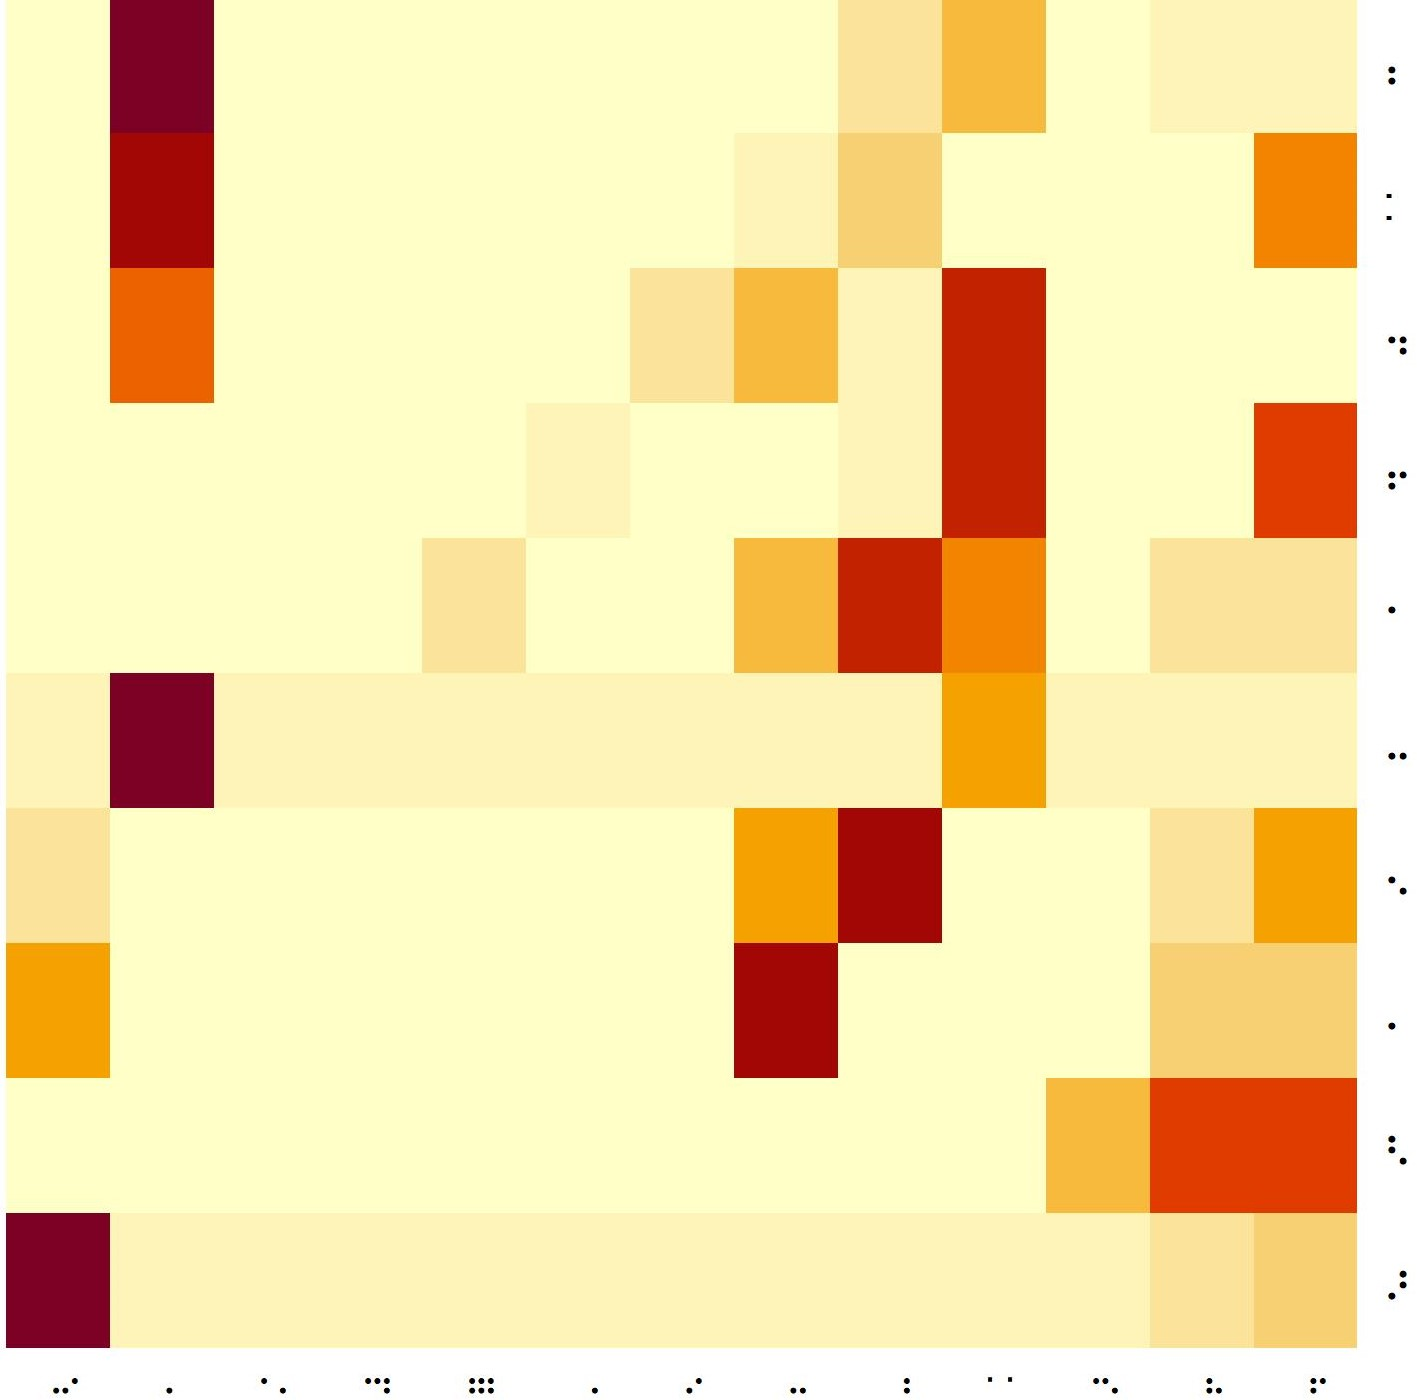
\includegraphics[width=\myPictWidth]{errors_stats/heatmap_special}
    \caption{Частоты замен знаков препинания на другие знаки препинания (по вертикали -- верный символ, по горизонтали -- распознанный). Цвет показывает долю исходных символов, приходящихся на заменяемый. Верно распознанные знаки не учтены.}
    \label{fig:heatmap_special}
\end{figure}

\newpage
\nonumsection{Приложение 2. Результаты подсчёта числа заменах букв в выравнивании}

\begin{table}[H]
    \centering
    \caption{Замены в тексте (показаны только символы, встретившиеся более 200 раз, и замены, частота которых превышает 0.05 от общего числа). (?) обозначает нераспознанный символ, * -- пропуск, XX -- знак вычеркнутой клетки (полное шеститочие).}
    \begin{tabular}{l p{.25\textwidth} l}
        \hline
        символ & число ошибочно распознанных вхождений & варианты замен (с указанием частоты) \\
        \hline
        o & 8289 & r: 0.92 \\
        n & 3638 & q: 0.74, *: 0.08 \\
        m & 2623 & p: 0.83 \\
        u & 1556 & v: 0.77, *: 0.07 \\
        d & 1406 & g: 0.51, e: 0.19, *: 0.1 \\
        a & 1190 & *: 0.36, b: 0.3, (?): 0.15, e: 0.06 \\
        ' & 1132 & <<: 0.95 \\
        s & 1124 & i: 0.46, *: 0.26, t: 0.13, p: 0.06 \\
        e & 1066 & h: 0.48, *: 0.32 \\
        y & 879 & XX: 0.53, *: 0.14, n: 0.11, (?): 0.08 \\
        , & 846 & *: 0.81 \\
        t & 839 & *: 0.3, j: 0.23, s: 0.17, 1: 0.07 \\
        h & 711 & e: 0.43, *: 0.35, ":": 0.08 \\
        k & 694 & l: 0.87, *: 0.06 \\
        l & 649 & *: 0.48, r: 0.18, (?): 0.1, b: 0.06 \\
        r & 426 & *: 0.34, h: 0.33, 1: 0.1 \\
        f & 415 & i: 0.43, *: 0.19, c: 0.11, b: 0.09 \\
        c & 395 & (?): 0.25, *: 0.23, f: 0.22, a: 0.12 \\
        8 & 351 & *: 0.8, <<: 0.07 \\
        i & 292 & *: 0.54, (?): 0.09, ":": 0.08 \\
        g & 265 & *: 0.21, h: 0.18, d: 0.15, f: 0.14 \\
        v & 237 & (?): 0.59, *: 0.14, r: 0.1 \\
        >> & 220 & <<: 0.29, 5: 0.14, (?): 0.09, ";": 0.06 \\
        << & 218 & 5: 0.26, *: 0.23, ': 0.19, 6: 0.06 \\
        x & 216 & (?): 0.76, *: 0.09 \\
        p & 213 & *: 0.41, s: 0.16, f: 0.07, q: 0.07 \\
        \hline
    \end{tabular}
    \label{table:per_letter_errs}
\end{table}

% TODO \ref{table:per_letter_errs}

\newpage
\nonumsection{Приложение 3. Исходный код программ}
Ниже приведён исходный код программы, реализующей модифицированный алгоритм Нидлмана-Вунша. % TODO ссылка на номер алгоритма
Этот код, а также программы, осуществляющие поиск регионов интереса, вспомогательные манипуляции с изображением (обрезка, переименование...) и текстом (замена символов, подсчёт статистик...) доступны в репозитории\footnote{\href{https://github.com/braille-systems/brl_data_tools}{github.com/braille-systems/brl\_data\_tools}}.
Там же можно найти инструкцию по установке и запуску, а также сслыки для загрузки файлов с исходными данными (файл \texttt{README.md}).

\lstinputlisting{../../scripts/needleman_wunsch.py}
\end{document}